\documentclass[a4paper,11pt,fleqn]{scrartcl}%fleqn pour aligner les equations à gauche
\usepackage{../../Styles/Cours}
%\usepackage{../../Styles/arduinoLanguage}


\usepackage{color}
\usepackage{mwe}
\usepackage{listings}    
\usepackage{etoolbox}    

\definecolor{mygreen}{rgb}{0,0.6,0}
\definecolor{mygray}{rgb}{0.47,0.47,0.33}
\definecolor{myorange}{rgb}{0.8,0.4,0}
\definecolor{mywhite}{rgb}{0.98,0.98,0.98}
\definecolor{myblue}{rgb}{0.01,0.61,0.98}

\newcommand*{\FormatDigit}[1]{\ttfamily\textcolor{mygreen}{#1}}
%% https://tex.stackexchange.com/questions/32174/listings-package-how-can-i-format-all-numbers
\lstdefinestyle{FormattedNumber}{%
    literate=*{0}{{\FormatDigit{0}}}{1}%
             {1}{{\FormatDigit{1}}}{1}%
             {2}{{\FormatDigit{2}}}{1}%
             {3}{{\FormatDigit{3}}}{1}%
             {4}{{\FormatDigit{4}}}{1}%
             {5}{{\FormatDigit{5}}}{1}%
             {6}{{\FormatDigit{6}}}{1}%
             {7}{{\FormatDigit{7}}}{1}%
             {8}{{\FormatDigit{8}}}{1}%
             {9}{{\FormatDigit{9}}}{1}%
             {.0}{{\FormatDigit{.0}}}{2}% Following is to ensure that only periods
             {.1}{{\FormatDigit{.1}}}{2}% followed by a digit are changed.
             {.2}{{\FormatDigit{.2}}}{2}%
             {.3}{{\FormatDigit{.3}}}{2}%
             {.4}{{\FormatDigit{.4}}}{2}%
             {.5}{{\FormatDigit{.5}}}{2}%
             {.6}{{\FormatDigit{.6}}}{2}%
             {.7}{{\FormatDigit{.7}}}{2}%
             {.8}{{\FormatDigit{.8}}}{2}%
             {.9}{{\FormatDigit{.9}}}{2}%
             %{,}{{\FormatDigit{,}}{1}% depends if you want the "," in color
             {\ }{{ }}{1}% handle the space
             ,%
}


\lstset{%
  backgroundcolor=\color{mywhite},   
  basicstyle=\footnotesize,       
  breakatwhitespace=false,         
  breaklines=true,                 
  captionpos=b,                   
  commentstyle=\color{red},    
  deletekeywords={...},           
  escapeinside={\%*}{*)},          
  extendedchars=true,              
  frame=shadowbox,                    
  keepspaces=true,                 
  keywordstyle=\color{myorange},       
  language=Octave,                
  morekeywords={*,...},            
  numbers=left,                    
  numbersep=5pt,                   
  numberstyle=\tiny\color{mygray}, 
  rulecolor=\color{black},         
  rulesepcolor=\color{myblue},
  showspaces=false,                
  showstringspaces=false,          
  showtabs=false,                  
  stepnumber=2,                    
  stringstyle=\color{myorange},    
  tabsize=2,                       
  title=\lstname,
  emphstyle=\bfseries\color{blue},%  style for emph={} 
}    

%% language specific settings:
\lstdefinestyle{Arduino}{%
    style=FormattedNumber,
    keywords={void},%                 define keywords
    morecomment=[l]{//},%             treat // as comments
    morecomment=[s]{/*}{*/},%         define /* ... */ comments
    emph={HIGH, OUTPUT, LOW},%        keywords to emphasize
}

\newtoggle{InString}{}% Keep track of if we are within a string
\togglefalse{InString}% Assume not initally in string


\newcommand{\chnum}{Chapitre 21}
\newcommand{\chtitle}{Détermination des caractéristiques d'un dipole RC avec un micro-contrôleur}
\newcommand{\dtype}{TP}


\begin{document}
	\maketitle

Objectifs : Déterminer expérimentalement le temps caractéristique d'un dipôle $RC$ à l'aide d'un microcontrôleur.

\begin{figure}[h!]
		\caption{Montage à réaliser}
		\begin{minipage}{.6\linewidth}
			La borne D2 peut être portée à +\SI{5}{V} pour charger le condensateur. ou à \SI{0}{V} pour le décharger.\\
			La borne A0 permet de mesurer la tension aux bornes du condensateur. Elle donne une valeur numérique de la tension. Elle peut comprendre $2^{10} = 1024$ valeurs différentes comprises entre 0 (correspondant à \SI{0}{V}) et 1023 (correspondant à \SI{5}{V}).\\
			Le montage sera réalisé via un simulateur en ligne.
		\end{minipage}
		\begin{minipage}{.3\linewidth}
			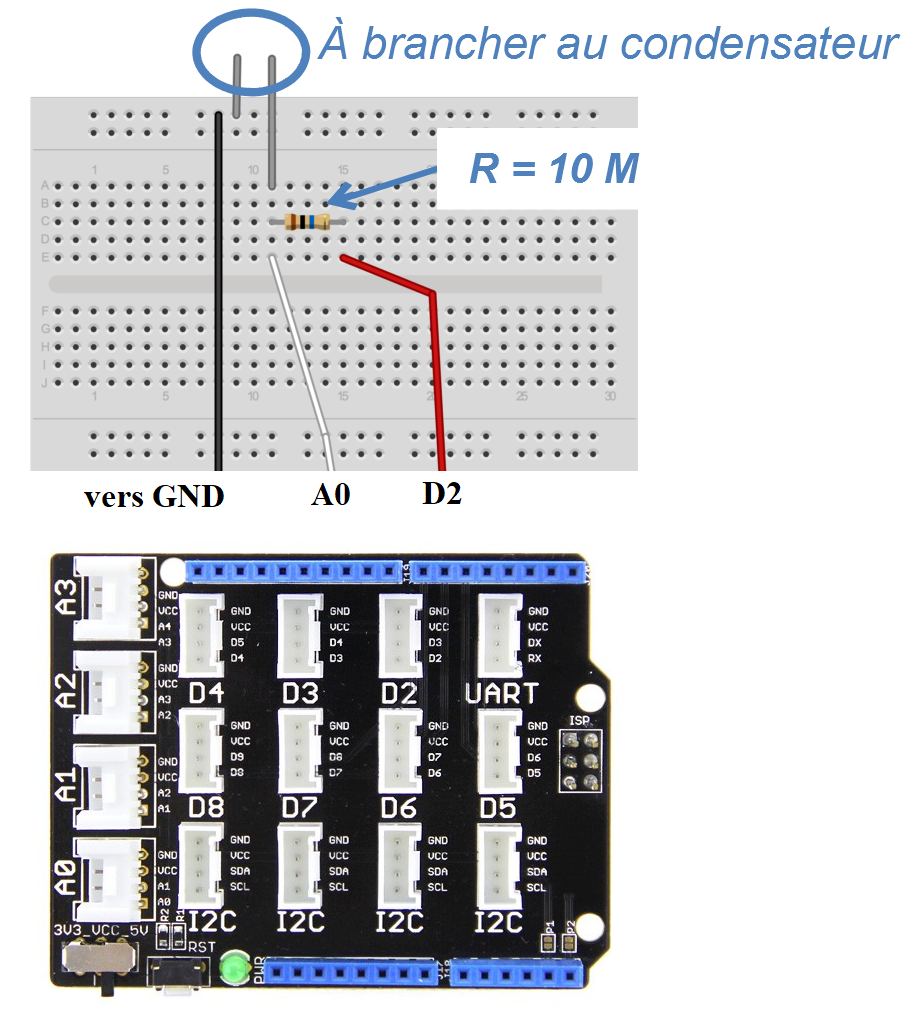
\includegraphics[scale = .2]{Ressources/TSPE_C11_AE2_Fig1.png}
		\end{minipage}
	\end{figure}

\begin{figure}[h!]
	\caption{Lancement du programme Ardiuno}
	\begin{minipage}{.9\linewidth}
		\begin{itemize}
			\item Télécharger le fichier code "TSPE\_TauRC.ino" dans votre dossier personnel.
			\item Ouvrir le programme
			\item Recréer un circuit ci-dessus
			\item Suivez les indications du document 1 pour les connections
			\item Ouvrir l'onglet "Code" et coller le contenu du fichier "TSPE\_TauRC.ino"
			\item Lancer la simulation
		\end{itemize}
	\end{minipage}
\end{figure}

\textbf{Questions}\\
	Les lignes 1 à 11 définissent les variables qui seront utilisées par le programme.
	\begin{enumerate}
		\item En ligne 10, la variable $R$ prend la valeur de la résistance, quelle est son unité ?\\
		Les lignes 16 et 17 préparent l'écriture des résultats dans le moniteur série.\\
		La ligne 18 lance une boucle "for" qui va réaliser 10 fois les instructions comprises entre les lignes 18 et 30.
		\item Expliquer pourquoi les lignes 20 à 22 permettent de décharger le condensateur.\\
		La fonction millis() est une fonction "chronomètre" : elle prend la valeur de la durée écoulée depuis le lancement du programme (ou depuis l'appui sur reset) en millisecondes.
		\item Le circuit n'a pas d'interrupteur, mais la ligne 25 peut être comparée à une action dur un interrupteur : quelle en serait l'action ?
		\item En ligne 27, on attend que la valeur lue sur la borne A0 dépasse 647, pourquoi cette valeur ?
		\item Expliquer pourquoi en ligne 30, la variable "tau" prendra la valeur du temps caractéristique du circuit en millisecondes.
		\item Quand on arrivera à la 10$^e$ répétition de la boucle, qui contiendra la variable nommée "tau10" ?
		\item Quel est l'intérêt de faire cette boucle de 10 mesures ?
		\item Justifier que les lignes 33 et 34 permettent d'obtenir la valeur de la capacité en nanofarad dans la variable C.
	\end{enumerate}

\begin{minipage}{.7\linewidth}
	\begin{lstlisting}[style=Arduino]
//broches
const int(Alim)=2;
const int(mesure) = A0;

//grandeurs
unsigned long debutCharge;
unsigned long tau;
unsigned long tau10 = 0;
float C;
float R = 10000000;
int i;

void setup()
{
// initialisation moniteur serie
  Serial.begin(9600);
  Serial.println("mesure...");
  for (i=0;i<10; i++){
// Decharge prealable de C (mise a 0V pendant 1s)
    pinMode (Alim, OUTPUT);
    digitalWrite (Alim, LOW);
    delay(1000); // attente d'une seconde
    
// Charge de C
    digitalWrite(Alim, HIGH);
    debutCharge=millis();
    while(analogRead(mesure)<647){
      //647 = 63% de 1023 on attend....
  }
    tau = millis() - debutCharge;
    tau10= tau10 + tau;
  }
  float (tau) = float(tau10)/10;
  float C = float(tau)*10000000/R; //C en nF
//affichage :
  Serial.print("Constante de temps : ");
  Serial.print(tau);
  Serial.println(" ms ");
  Serial.print("Capacite : ");
  Serial.print(C);
  Serial.println(" nF");
}
  void loop(){
}
	\end{lstlisting}
\end{minipage}

\end{document}